\documentclass[hidelinks,12pt]{article}
%\usepackage[italian]{babel}
\usepackage{natbib}
\usepackage{url}
\usepackage[utf8x]{inputenc}
\usepackage{amsmath}
\usepackage{graphicx}
\graphicspath{{images/}}
\usepackage{parskip}
\usepackage{hyperref}
\usepackage{fancyhdr}
\usepackage{scrextend}
\usepackage[T1]{fontenc}
\usepackage{vmargin}
\setmarginsrb{3 cm}{2.5 cm}{3 cm}{2.5 cm}{1 cm}{1.5 cm}{1 cm}{1.5 cm}

\title{Technical Manual}                             % Title
\author{Guido Pio Mariotti\\Giuliano Torrisi}                               % Author
\date{22 July 2016}                                           % Date

\makeatletter
\let\thetitle\@title
\let\theauthor\@author
\let\thedate\@date
\makeatother

\pagestyle{fancy}
\fancyhf{}
%\rhead{\theauthor}
\lhead{\thetitle}
\cfoot{\thepage}

\begin{document}

%%%%%%%%%%%%%%%%%%%%%%%%%%%%%%%%%%%%%%%%%%%%%%%%%%%%%%%%%%%%%%%%%%%%%%%%%%%%%%%%%%%%%%%%%

\begin{titlepage}
    \centering
    \vspace*{0.5 cm}
    
\includegraphics[scale = 0.35]{polito_logo.png}\\[1.0 cm]   % University Logo
    \textsc{\LARGE \textbf{Politecnico di Torino}}\\[2.0 cm]   % University Name
    \textsc{\Large Bioinformatics}\\[0.5 cm]               % Course Code
    %\textsc{\large Course Name}\\[0.5 cm]               % Course Name
    \rule{\linewidth}{0.2 mm} \\[0.4 cm]
    { \huge \bfseries \thetitle}\\
    \rule{\linewidth}{0.2 mm} \\[1.5 cm]
    \vspace{20 pt}
    \begin{minipage}{1\textwidth}
        \begin{flushright} \large
            \emph{\textbf{Authors}:}\\
            \theauthor
            \end{flushright}
    \end{minipage}\\[2 cm]
    {\large \thedate}\\[2 cm]
 
    \vfill
    
\end{titlepage}

%%%%%%%%%%%%%%%%%%%%%%%%%%%%%%%%%%%%%%%%%%%%%%%%%%%%%%%%%%%%%%%%%%%%%%%%%%%%%%%%%%%%%%%%%

\tableofcontents
\pagebreak

%%%%%%%%%%%%%%%%%%%%%%%%%%%%%%%%%%%%%%%%%%%%%%%%%%%%%%%%%%%%%%%%%%%%%%%%%%%%%%%%%%%%%%%%%

\section{Introduction}

GDC Data Portal gives the opportunity to download large amount of genomic data directly from the web or using the GDC Data Transfer Tool. 
This program allows users to manage only the files downloaded through GDC Data Transfer Tool.

Full compatibility: Python 2.7.\\
Compatibility: Python 2.6 if module argparse is installed.\\
Compatibility: Python 3.x if program 2to3 is used.

\section{Configuration}
\subsection{First Steps}
The first time you run the program, it is required to perform a quick configuration.
The only information needed is the directory with the downloaded GDC files, that from now on we will refer to as \textbf{GDC\_download\_dir}.
This information can be set at first program run, or using the terminal option "-d", as described in \textit{section 4.3}.
In order to have more flexibility, is important to insert an absolute path representing the downloads directory, but this is not mandatory, since the program still work even if the path is relative.\\
After you have created the configuration file, which will be put in the same location where the program is called, there will be two more options to manage it.
One is for updating the GDC\_download\_dir, using the corresponding option during execution or the terminal option \textbf{-u} (see \emph{section 4.4} for more information), the other one is the complete remove of the configuration file using the menu or \textbf{-rc} terminal option (\textit{section 4.5}).

\subsection{How to use the tool}

\begin{enumerate}
\item Add to GDC Data Portal cart all the files you want to download.
\item Go to cart page and, clicking on ``Download'' button, choose ``Manifest'' and ``File Metadata''. These files must be copied in the folder chosen during configuration. Manifest are plain text files, while Metadata are json files.
\item From the ``GDC\_download\_dir'', use the GDC Data Transfer Tool to obtain all the files previously selected on the portal. For each file, a new directory will be created using as name the file's "UUID".
\item Start the tool and something like the image below will be prompted.

%, after the first listing, all the directories will be renamed in a more readable way (refer %to section "Rename Directories" of chapter "Functionalities" to have more information about %the name used).
\end{enumerate}

\vspace{20 pt}
\begin{center}
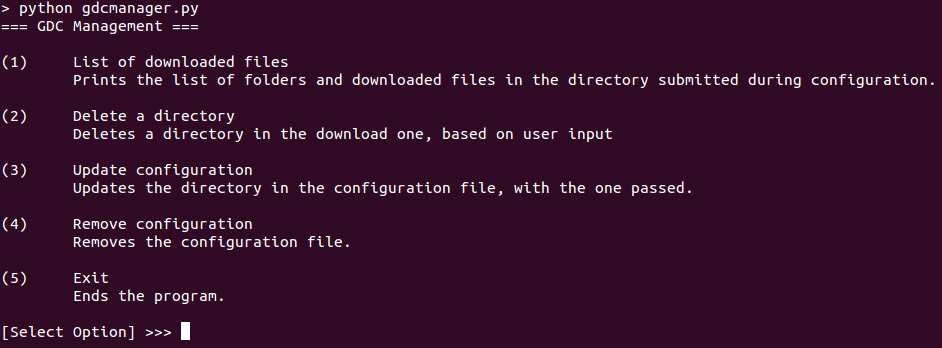
\includegraphics[scale = 0.45]{menu_picture.png}\\[0.5 cm]
\end{center}

%%%%%%%%%%%%%%%%%%%%%%%%%%% FUNCTIONALITIES  %%%%%%%%%%%%%%%%%%%%%%%%%%%%%%%%%%%%%%%%

\section{Functionalities}

%%%%%%%%%%%%%%%%%% RENAME DIRECTORIES %%%%%%%%%%%%%%%%%%%%%%%%%

\subsection{Rename Directories}
Files downloaded through GDC Data Transfer Tool are saved into a directory (one per file) named as the "UUID" of the data. To each file is associated a name and one or more "entity\_submitter\_id". These information can be found respectively in Manifest and Metadata files.\\
The program will rename directories using a concatenation between part of the entity\_submitter\_id and the file name.
For the sake of clarification, we can consider the following example:\\

Suppose you want to download the following files:

\begin{footnotesize}

\begin{itemize}
\item \textbf{File 1}:
	\begin{itemize}
	\item UUID: ``32e84d8b-4132-4aab-8f10-3f78f777e27e''
	\item File\_name: ``00eb7c26-84fd-4ab9-93a1-3d209dfc0f43.FPKM.txt''
	\item Entity\_submitter\_id: ``TCGA-M7-A720-01A''
	\end{itemize}
\end{itemize}



\begin{itemize}
\item \textbf{File 2}:
	\begin{itemize}
	\item UUID: ``ed77b3cf-a543-439f-8e11-7c1fb9efb157''
	\item File\_name: ``006cb4e4-cb57-4b4f-98ed-475fa7f7f74d\_gdc\_realn\_rehead.bam''
	\item Entity\_submitter\_id: ``TCGA-A6-2686-01A''
	\end{itemize}
\end{itemize}
	
\end{footnotesize}

\clearpage

After the download with GDC Data Transfer Tool, you will find two directories with names:

\begin{footnotesize}
\begin{enumerate}
\item ``32e84d8b-4132-4aab-8f10-3f78f777e27e''
\item ``ed77b3cf-a543-439f-8e11-7c1fb9efb157''
\end{enumerate}
\end{footnotesize}

The tool will rename all of them concatenating the entity submitter id with the file name, with, as separator, an underscore (\_). \\ The result will be: 
\begin{footnotesize}
\begin{enumerate}
\item ``TCGA-M7-A720-01A\_00eb7c26-84fd-4ab9-93a1-3d209dfc0f43.FPKM''
\item ``TCGA-A6-2686-01A\_006cb4e4-cb57-4b4f-98ed-475fa7f7f74d\_gdc\_realn\_rehead''
\end{enumerate}
\end{footnotesize}

Directories will be renamed in three cases:
\begin{itemize}
\item Option ``List Directories'' chosen (explained in \textit{section 3.2})
\item Command line option \textbf{-s} or \textbf{--scan} chosen (explained in \textit{section 4.1})
\item Command line option \textbf{-l} or \textbf{--listing} chosen (explained in \textit{section 4.2})
\end{itemize}

\paragraph{Manifest and Metadata files}
The Manifest and Metadata files which have already been used to download data are moved to an hidden directory that works as a cache. This can be found inside ``GDC\_download\_dir'' under the name ``.cache\_gdc''.
Furthermore for each file a new hidden manifest is created in the same directory, containing all the information related to that file. 

\paragraph{Compressed Files}
Some files downloaded from the GDC Data Portal are compressed. The program will automatically detect and uncompress them.


%%%%%%%%%%%%%%%%%% LIST DIRECTORIES %%%%%%%%%%%%%%%%%%%%%%%%%  

\subsection{List Directories}
List all directories present in the main folder in alphabetic order. For each one is also printed the contained file.\\
The program verifies automatically that all the directories have been renamed and in case run the renaming process, before listing.

%%%%%%%%%%%%%%%%%% DELETE FOLDER %%%%%%%%%%%%%%%%%%%%%%%%%

\subsection{Delete Folder}

This option will allow you to remove a directory, and its content, from the GDC\_download\_dir.
First, the list of all the directories, and files inside of them, will be printed in alphabetical order on screen, with a number associated to each directory. Once the list has been printed, you will be prompted to insert the number associated to the directory you want to delete.\\
Deletion is permanent, and the number associated to each directory is not hardcoded with it, so be careful.

%%%%%%%%%%%%%%%%%% MANAGE CONFIGURATIONS %%%%%%%%%%%%%%%%%%%%%%%%%

\subsection{Update Configuration}
This option will allow you to update the configuration file created during the first steps. You will be prompted to insert the new directory in order to update the configuration file. The directory must be a valid absolute or relative path.

\subsection{Delete Configuration}

This option will allow you to remove the configuration file created the first time.
You will be prompted to insert a new directory in order to create a new configuration and then you will have the possibility
to select an option from the menu. \\
If you are not interested in creating a new configuration, refer to the terminal option \textbf{-rc} as explained in \textit{section 4.3}

\clearpage

%%%%%%%%%%%%%%%%%% COMMAND OPTIONS %%%%%%%%%%%%%%%%%%%%%%%%%

\section{Command Options}

You can execute all the functionalities of the tool passing options from command line.\\

\textbf{Synopsis:}
\begin{center}
\textbf{gdcmanager [options]}
\end{center}

\begin{center}
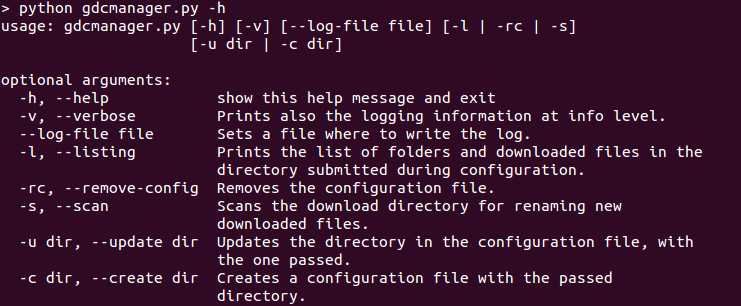
\includegraphics[scale = 0.6]{help_picture.png}\\[0.5 cm]
\end{center}

%%%%%%%%%%%%%%%%%%%%%%%%%%%%%%%%%%%%%%%%%%%%%%%%%%%%%%%%%%%%%%%

\subsection{Rename Directories}
\textbf{Command option:} ``-s'' or ``-\hspace{0.1 pt}-scan''
\vspace{10 pt}
\\Can be used with -d and -u\\
This option allows you to perform just scanning and renaming of the downloaded directories, without the listing, as, 
instead, happens with the -l option.

%%%%%%%%%%%%%%%%%%%%%%%%%%%%%%%%%%%%%%%%%%%%%%%%%%%%%%%%%%%%%%%

\subsection{List Directories}
\textbf{Command option:} ``-l'' or ``-\hspace{0.1 pt}-listing''
\vspace{10 pt}
\\Can be used with: -d and -u \\
List directories and each contained files in alphabetic order. If new files have been downloaded before the last listing, the relative directories will be renamed and the new names printed.


%%%%%%%%%%%%%%%%%%%%%%%%%%%%%%%%%%%%%%%%%%%%%%%%%%%%%%%%%%%%%%%

\subsection{Create Configuration}
\textbf{Command option:} ``-d <dir>'' or ``-\hspace{0.1 pt}-directory <dir>''
\vspace{10 pt}
\\Can be used with: -l, -rc and -s\\
This option allows you to create the configuration file using the directory passed as argument. \\ It will work only if the directory is valid. If the configuration already exist, a message to suggest the use of -u will be print.

%%%%%%%%%%%%%%%%%%%%%%%%%%%%%%%%%%%%%%%%%%%%%%%%%%%%%%%%%%%%%%%

\subsection{Update Configuration}
\textbf{Command option:} ``-u <dir>'' or ``-\hspace{0.1 pt}-update <dir>''
\vspace{10 pt}
\\Can be used with: -l, -rc and -s\\
This option allows you to update the GDC\_download\_dir in the configuration file with the one passed as argument, working exactly as the option in \textit{section 3.4}. \\ It will work only if the directory is valid. If the configuration doesn't exist, a message to suggest the use of -d will be print.

%%%%%%%%%%%%%%%%%%%%%%%%%%%%%%%%%%%%%%%%%%%%%%%%%%%%%%%%%%%%%%%

\subsection{Delete Configuration}
\textbf{Command option:} ``-rc'' or ``-\hspace{0.1 pt}-remove-config''
\vspace{10 pt}
\\Can be used with: -d and -u\\
The option is the same as the one explained in Delete Folder \textit{section 3.3} but it will prompt you with the request of a new directory for the configuration file.\\ Use this only if you want to quickly remove the configuration.
%%%%%%%%%%%%%%%%%%%%%%%%%%%%%%%%%%%%%%%%%%%%%%%%%%%%%%%%%%%%%%%

\subsection{Log Configuration}
\textbf{Command option:} ``-v'' or ``-\hspace{0.1 pt}-verbose''\\
\textbf{Command option:} ``-\hspace{0.1 pt}-log-file'' <file>
\vspace{10 pt}
\\Can be used with: -s -l -rc -d and -u\\
The options give the possibility to modify log output. Default configuration will show only errors from WARNING level, without saving into a file.\\
The -v or -\hspace{0.1 pt}-verbose set the log level to INFO, printing all messages from the logger.
The -\hspace{0.1 pt}-log-file gives the possibility to save the log on a file.

\clearpage

%%%%%%%%%%%%%%%%%%%%% ISSUES AND SOLUTIONS %%%%%%%%%%%%%%%%%%%%

\section{Issues and solutions}

%%%%%%%%%%%%%%%%%%%%%%%%%%%%%%%%%%%%%%%%%%%%%%%%%%%%%%%%%%%%%%%

\subsection{Configuration file management}
In order to implement an easy to improve solution, we have decided to use a .ini file. Like most of the file extension, Python offers ConfigParser class in order to perform the parsing and the serialization of the file. This class is present in Python 2.6 and 2.7 but can be easily converted for Python 3.5 using the tool 2to3 offered by the Python Organization.
The configuration file has just a section and a <key:value> pair in order to store the directory inserted by the user at creation time. For future versions of the program, new configuration values can be easily inserted in the Configuration 
class file in order to add new functionalities.
Look at ``Configuration'' section in ``Possible Improvements'' for future modifications.

%%%%%%%%%%%%%%%%%%%%%%%%%%%%%%%%%%%%%%%%%%%%%%%%%%%%%%%%%%%%%%%

\subsection{Manage all downloaded files}
One of the main problem we had to face with, was how to manage the list of all the files present in our directory. \\ In order to do that we have decided to create a file, named ``MANIFEST.txt'', where we store all the information regarding each file and the name of the folder that contains it.\\
For each file we save all the info read from the manifest downloaded from the GDC Data Portal and the entity\_submitter\_id read from the metadata file.

%%%%%%%%%%%%%%%%%%%%%%%%%%%%%%%%%%%%%%%%%%%%%%%%%%%%%%%%%%%%%%%

\subsection{User deletes a folder manually}
In order to handle situations in which a user has deleted manually a folder inside GDC\_download\_dir, we check if our current version of the ``MANIFEST.txt'' is compliant with the current state of the folder. If one of the file present in our manifest is no longer available, we delete the entry and update the manifest. This process will be executed all the time that we try to list all the available folders and files.

%%%%%%%%%%%%%%%%%%%%%%%%%%%%%%%%%%%%%%%%%%%%%%%%%%%%%%%%%%%%%%%

\subsection{Compressed Files}
We realized that, in some cases, files downloaded from GDC Data Portal are compressed with ``.gz'' extension. In order to give the possibility to the user to work with them directly, we decided to uncompress them as soon as we scan the GDC\_download\_dir to rename all the folders.

%%%%%%%%%%%%%%%%%%%%%%%%%%%%%%%%%%%%%%%%%%%%%%%%%%%%%%%%%%%%

\subsection{Clear the working folder}
Every time a manifest or a metadata is used to download files, it will remain in the same folder until the user will delete it, creating useless garbage. \\
In order to face with this problem, during the rename process we move all the manifest and metadata files previously downloaded to an hidden folder named ``.cache\_gdc'', located in GDC\_download\_dir, and prepend to the manifest or metadata names the string ``done\_''. This way the user will be able to recollect them if needed.\\ 
Furthermore in case one of the downloaded manifest or metadata has not been used yet, it will not be moved to the cache\_gdc dir, to allow later use.

%%%%%%%%%%%%%%%%%%%%%%%%%%%%%%%%%%%%%%%%%%%%%%%%%%%%%%%%%%%%%%%%%%

\subsection{Getting the entity submitter id for each file}
During renaming process we retrieve, from the metadata, information on the submitter id of each file, in order to make the name of the folder more readable and to allow each user to link files with related associated entities. \\ To do that we have used the json python module to read and retrieve information from each metadata file. One of the problem we had to face with was the fact that we could have more than one associated entity and we could not be sure on which one take into account. So we took only the first that we encounter. \\Anyway it is very easy to modify the code in order to let the program read another id. 

%%%%%%%%%%%%%%%%%%%%%%%%%%%%%%%%%%%%%%%%%%%%%%%%%%%%%%%%%%%%%%%%%%

\subsection{Menu visualization and Option selection}
We have implemented a Menu class to visualize and execute one of the multiple functionalities of the program. To do that while
allowing the possibility of future options to be inserted, the Menu object takes as parameter one or more Option objects.
Each Option takes as parameter the title of the function, a comment to it and a callable object, that will be called when the option is selected. In order to add new functionalities to the program, is enough to create a class that implements the \underline{\hspace{0.4cm}}call\underline{\hspace{0.4cm}} method, or simply passing a function pointer to it. 


\section{Possible improvements}

\subsection{Configuration}
\begin{itemize}
\item Multiple directories in order to allow the user to set more than one directory as root for GDC downloaded files.
\end{itemize}

\subsection{Delete Folder}
\begin{itemize}
\item Terminal option  that accept the name of the directory, or a list of directories, to be deleted.
\end{itemize}

\subsection{Uncompress Files}
\begin{itemize}
\item The program can also handle compressed files with ``zip'' extension, even if GDC Data Portal does not seem to send files to the user in this format. A possible improvement could be to read the compressed file in chunks to avoid uncontrolled memory consumption (this has been already implemented for ``gz'' extension). 
\end{itemize}











\end{document}